\documentclass{beamer}

\usepackage[utf8]{inputenc}
\usepackage[T1]{fontenc}

\title{Projet tremplin 2020}
\author{}
\date{Vendredi 4 septembre 2020}


\begin{document}

\frame{
  \maketitle
}

\frame{
  \frametitle{On fait quoi ce matin ?}

  \begin{block}{Un concours de résolution de labyrinthes}
    \begin{itemize}
    \item Arènes imposées à construire (12x12)
    \item Toujours les mêmes points de départ (0,0) et d'arrivée (11,11)
    \item 45 minutes de concours, 1h de préparation
    \end{itemize}
    \textcolor{red}{\bf Objectif~:} en résoudre le plus possible
  \end{block}

}

\frame{
  \frametitle{En pratique}

  \begin{block}{Tout le monde part avec le même labyrinthe (très difficile)}

    \begin{center}
    \begin{tabular}{|c|c|c|}
      \hline
      0 & 0 & 0 \\
      \hline
      0 & 0 & 0 \\
      \hline
      0 & 0 & 0 \\
      \hline
    \end{tabular}

    \vspace*{0.5cm}

    \fbox{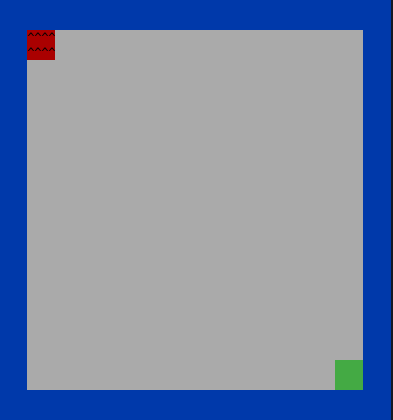
\includegraphics[width=4.5cm]{lab1.png}}
    \end{center}

  \end{block}


}

\frame{
  \frametitle{En pratique 2}

  \begin{block}{Une fois résolu un labyrinthe on le signale}

    \begin{center}
      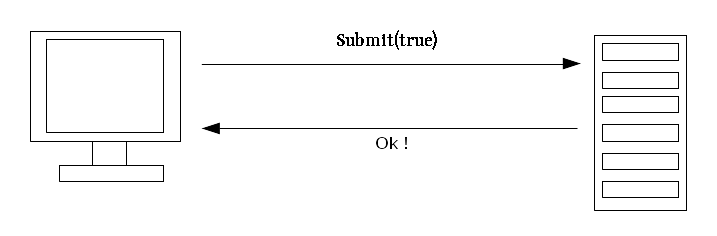
\includegraphics[width=10cm]{soum.png}
    \end{center}

    \textcolor{red}{Résolu~:} être à l'arrivée ou avoir détecté que c'est impossible

  \end{block}

}

\frame{
  \frametitle{En pratique 3}

  \begin{block}{On obtient un nouveau labyrinthe}
    \hfill (ou le même si on s'est trompé)


    \centering
    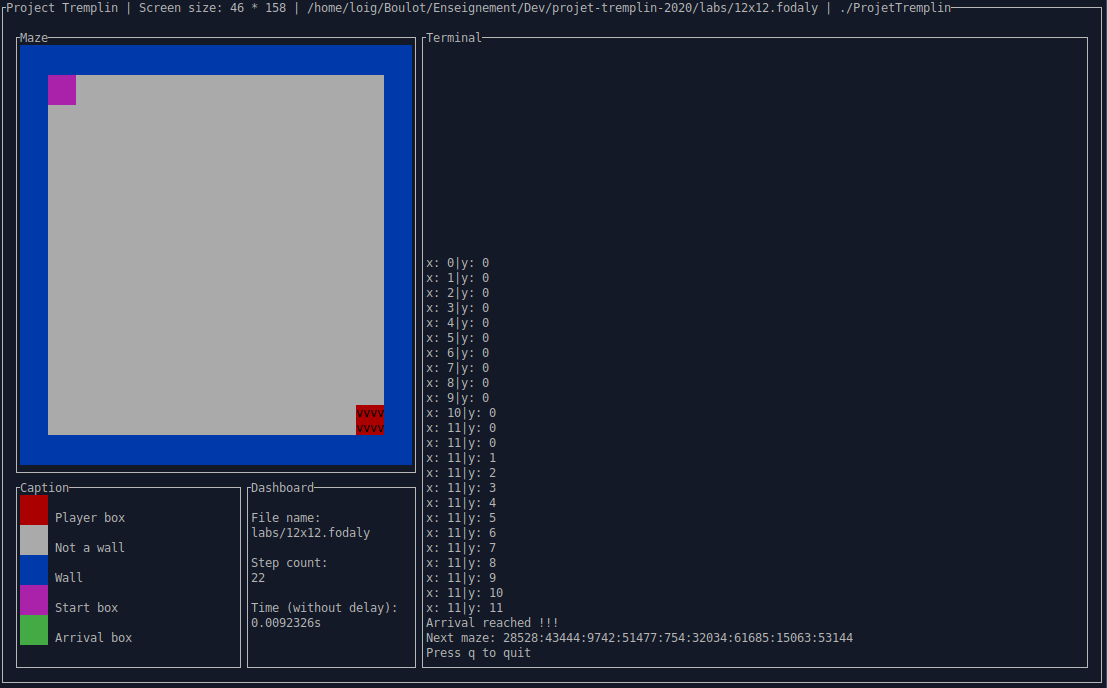
\includegraphics[width=11cm]{nouveau.png}

  \end{block}

}

%\frame{
%  \frametitle{La nouvelle bibliothèque liblabyrinthes.a}
%
%  \begin{block}{Où la trouver ?}
%    Sur Madoc, dès la fin de cet amphi
%  \end{block}
%
%  \begin{block}{Quels fichiers}
%    \begin{itemize}
%    \item liblabyrinthes.a
%    \item labyrinthes.h
%    \end{itemize}
%  \end{block}
%
%  \begin{block}{Quoi de neuf ?}
%    Une fonction de plus : submit
%  \end{block}
%
%}

\frame{
  \frametitle{La fonction submit}

  \begin{center}

    \Large submit(solvable)

  \end{center}

  \begin{block}{Paramètre}
    \begin{itemize}
    \item \textcolor{blue}{\bf solvable~:} true si le labyrinthe a une solution, false sinon
    \end{itemize}
  \end{block}

  \begin{block}{Valeur de retour}
    \begin{itemize}
      \item \textcolor{blue}{\bf 0~:} tout s'est bien passé
      \item \textcolor{blue}{\bf 1~:} mauvais labyrinthe
      \item \textcolor{blue}{\bf 2~:} mauvais identifiant ou mauvais serveur
      \item \textcolor{blue}{\bf autre~:} erreur réseau, me le signaler
    \end{itemize}
  \end{block}

  \textcolor{red}{\bf Ceci est rappelé dans labs.h}

}

\frame{
  \frametitle{Attention}


    \begin{block}{Utilisation du programme}
      \begin{itemize}
      %\item move vs. do\_move
      \item utiliser le mode "contest" (--contest user@server)\\

      \item<2-> penser qu'on n'est pas obligé d'afficher les labyrinthes pour les résoudre (-d 9)
      \end{itemize}
    \end{block}

  \begin{block}{Serveurs}
    \begin{itemize}
    \item adresses utilisées les autres jours
    \item mêmes identifiants
    \end{itemize}
  \end{block}


}

\frame{

  \centering
  \Huge

  Des questions ?

}

\frame{
  \frametitle{Et après ?}

  \begin{block}{D'ici quelques jours}
    \begin{itemize}
    \item Résultat individuel par mail
    \item Résultats (anonymisés) de la promo entière
    \end{itemize}
  \end{block}

}

\frame{

  {\centering
  \Huge

  Au boulot !
  }

  \vspace*{0.5cm}

  \begin{block}{Jusqu'à 11h, serveurs en route}
    Testez submit (signalez les problèmes !)
  \end{block}

  \begin{block}{À 11h15, remise à zéro des serveurs}
    45 minutes pour résoudre le plus de labyrinthes possible
  \end{block}

}

\end{document}
